\chapter{Introduction}

The Standard Model (SM) of particle physics has been phenomenally successful in describing all of the observed fundamental particles and their interactions. Its predictive powers have been made evidently manifest with the discovery of the Higgs boson in 2012 at the Large Hadron Collider (LHC) at CERN \cite{collaborationObservationNewBoson2012}, as well as with the discovery of the top quark at the Tevatron at Fermilab in 1995 \cite{abachiObservationTopQuark1995}. In fact, eight of the fundamental particles that conform to the SM were predicted to exist before their eventual discovery. However, despite its success, there is clear evidence that it does not a constitute a complete theory \cite{saikumarExploringFrontiersChallenges2024,garrettDarkMatterPrimer2011}: the matter-antimatter asymmetry, the neutrino's non-zero mass, the hierarchy problem, the fine-tuning problem of the Higgs, and the inability of this framework to describe gravity. This work, however, will focus on a particularly compelling sign of this theory's incompleteness: the existence and abudance of dark matter.

Dark matter (DM) is a form of non-baryonic matter that does not interact through any of the forces described by the SM (i.e., the electromagnetic, weak, and strong forces), and its presence can only be inferred through its gravitational influence. The first signs of its existence can be traced back to J.H. Oort's observations in the early 1930s that the velocity distribution of stars in the Milky Way is such that stars should be moving fast enough to escape the gravitational grasp of the observable mass. He postulated that a possible explanation (beyond error) is that there is a significant amount of non-luminous matter deepening the gravitational well of the galaxy, holding these stars in their orbits. Later studies by V. Rubin in the 1980s of the rotation curves of 60 spiral galaxies showed that the extent of the galaxy's mass was much larger than what could be attributed to the visible matter.

However, the evidence for dark matter is not limited to the rotation curves of galaxies. The relatively small scale of the anisotropies observed in the Cosmic Microwave Background (CMB) by COBE (COsmic Background Explorer) are too small to have been the seeds of the formation of large-scale structures in the universe. There must have been a charge-neutral matter that was able to start the structural formation before recombination happened in the early universe. Precision studies of the CMB fluctuations carried out using WMAP (Wilkinson Microwave Anisotropy Probe) have indicated that the total matter density of the universe is $\Omega_{m}h^2 = 0.1334$, and that only a small fraction of this, $\Omega_{b}h^2 = 0.02260$, is attributable to baryonic matter. The rest, $\Omega_{dm}h^2 = 0.1123$ or about $83\%$ of the total mass density, comes from the elusive dark matter. Thus, a substantial amount of the universe's content is non-baryonic and not described by the SM.

Numerous models have been proposed to extend the Standard Model to accomodate DM. Among them are supersymmetry and WIMPs, but no signs of these have been observed. Another class of models of particular interest in this work are those that propose that dark matter is composed of stable dark baryons in a confining Hidden Valley sector that interacts with the SM only through a mediator. If we assume the cogeneration of dark matter and baryonic matter in the early universe through the same mechanism, then we could simultaneously explain the matter-antimatter asymmetry, the dark matter abundance, and the coincidence of mass and number density of DM and baryonic matter. Moreover, this class of models would be consistent with astronomical observations indicating that dark matter is cold and has large self-interactions.

We consider the class of dark sector models with a TeV-scale mediator. For this class of models, when the dark quarks are produced, their energies will be higher than the confinment scale $\Lambda_D$ of the dark guague group, resulting in the hadronization of dark quarks into dark hadrons. Assuming the dark sector is QCD-like, this process will produce dark jets. Some of the dark hadrons forming part of these jets could be unstable and decay back into SM particles. If we consider the lifetime of these particles to be long, they would travel a potentially macroscopic distance before decaying, producing a detectible particle shower. Because this decay would be a stochastic process, the energy from the dark jet would \textit{emerge} into our detector as the dark hadrons decay back into detectable SM particles. This emerging jet (EMJ) would have be wide and have a displaced vertex, and their detection would serve as a smoking gun for composite dark sector models. Figure \ref{fig:emj} shows a schematic depiction of what such objects might look like in our detector.

% TODO: MAKE MY OWN GRAPHIC AND INCLUDE HERE
\begin{figure}[ht]
	\centering
	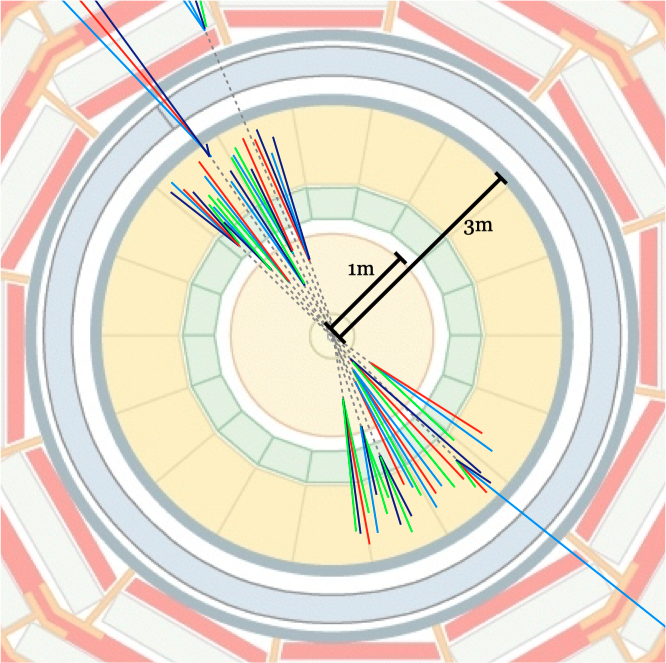
\includegraphics[width=0.5\textwidth]{images/emj.png}
	\caption{Schematic depiction of two EMJs produced through the pair production of dark quarks. The dark quarks hadronize into dark hadrons, some of which are unstable and decay back into SM particles after some distance. The energy from these decays emerges into the detector, producing a wide jet with a displaced vertex.}
	\label{fig:emj}
\end{figure}

% EMJs at the LHC
Previous searches for EMJs at the Large Hadron Colldier have focused on models with dark meson lifetimes inside the tracker volume of the CMS detector\footnote{There have been no dedicated searches for EMJs in ATLAS.}. Moreover, since there was no dedicated EMJ trigger, these searches used triggers that cut on the scalar sum of transverse momenta of jets, or $H_T$. Events with high jet activity would be selected, particularly for the models considered in these searches which focused on the pair production of bi-fundamental scalar mediators leading to the production of two EMJs and two QCD jets.

Having set the most stringent limits on these models, the next phase of the analysis looks towards the inclusion of models in which the mediator is a neutral vector boson, which leads to the production of just two EMJs. This new model leads to signals that are more difficult to find, as the EMJs are softer and the multi-jet QCD background would dominate. In addition to a new mediator, the next phase of the search looks to include models with longer-lived dark pions, such that they would mostly decay outside of the tracker volume.

With these new domains in sight for the Run 3 era of the analysis, a new trigger strategy is needed to effectively increase the sensitivity. In this work, we present trigger efficiency results for a set of novel triggers, namely machine learning (ML) based anomaly detection (AD) triggers and long-lived particle (LLP) triggers.

In Chapter 2 of this work, we will review the Standard Model of particle physics and the specifics of the dark sector models under consideration. In Chapter 3, an overview of the CMS detector will be provided, with particular focus on Run 3 upgrades to the calorimeters and the trigger system. In Chapter 4, a discussion of the event generation for the samples used in these studies is discussed. In Chapter 5, we present the results of the trigger efficiency studies for the novel triggers. Finally, in Chapter 6, we present the prospects for the Run 3 phase of the EMJ analysis and the future of the search for EMJs at the LHC.

% Scratch area:

% In this work we focus on the case where the confinment scale of the dark sector falls well below the center of mass energy of the LHC, i.e. $\Lambda_{\text{D}} \ll \sqrt{s}$. In such a case, dark quarks would be produced in the LHC, shortly before hadronizing into dark hadrons. Some fraction of these dark hadrons would be stable and thus serve as dark matter candidates. Others, however, would decay back into SM particles. The phenomenology of such a models is rich and so many of the searches taking place at the LHC focus on the exotic signatures predicted, without neccesity for a strong theory prior. Among the many of these types of signatures a dark sector might produce, we have emerging jets.

% % Emerging jets
% Emerging jets (EMJs) are a type of signature that arises when a dark jet is produced in the LHC following the production of dark quarks. Some of the particles in these invisible jets might escape our detector. However, unstable dark mesons (i.e. $\pi_{\text{dark}}$, $\rho_{\text{dark}}$) could travel some potentially macroscopic distance before decaying back into SM particles, producing a detectible particle shower. Given that the process of these dark mesons decaying into SM particles is a stochastic process, the location of the decay is distributed, meaning that the energy from this jet emerges into our detector, resulting in a wide jet with a displaced vertex.


% The universe's overall matter energy density in the universe is $\Omega_{m} \sim 0.32$. Of this, only a staggeringly small $\Omega_{\text{B}} \sim 0.05$ is attributable to baryonic matter. The other $\Omega_{\text{DM}} \sim 0.27$ is beyond the scope of the SM, as it is constituted by a type of matter which does not interact with baryonic matter through any of the known forces, and is only detectable through its gravitational influence. Signs of this dark matter were first observed in the early 1930s by J.H. Oort from the velocity distributions of stars relative to their distance from the Milky Way, and the first strong postulation of the domination of non-luminous matter surrounding galaxies was put forward by V. Rubin in the 1980s \cite{} when observations of the rotation curves of 60 spiral galaxies indicated that the extent of the galaxy's mass was much larger than what could be accounted for by visible matter \cite{}. This, however, was just the first sign of the dominance of dark matter. Cosmic microwave background anisotropies serving as indicators of the presence of a charge neutral matter that jump started the formation of structures in the early universe before recombination, numerous examples of gravitational lensing much stronger than what can be accounted for using visible baryonic matter, as well as examples where the baryonic and dark matter separate, such as the Bullet Cluster, all point to a form of matter that is wholly beyond the current scope of the SM. This demands a more complete theory.


% The Standard Model of particle physics has been phenomenally succesful in describing all observed fundamental particles and their interactions. Its predictive power has been repeatedly demonstrated, such as in 2012 with the discovery of the Higgs boson at the Large Hadron Collider (LHC) at CERN \cite{collaborationObservationNewBoson2012}, as well as with the discovery of the top quark at the Tevatron in 1995 \cite{abachiObservationTopQuark1995}. Despite its success, there exists an abundance of signs that the Standard Model is an incomplete theory. Among these, we have the matter-antimatter asymmetry in the universe \cite{}, the existence of dark matter, the neutrino's non-zero mass, the lightness of the Higgs boson \cite{saikumarExploringFrontiersChallenges2024}, and the inability to describe gravity within this framework \cite{}.

% Dark matter
% Of particular interest in this work is the elusive dark matter. Evidence for this type of matter, which does not interact with baryonic matter through any of the known forces except the gravitaional force, is abundant. Among this evidence, we have the cosmic microwave background anisotropies, graviational lensing, and the rotation curves of galaxies \cite{}. From these pieces of evidence, we have come to the conclusion that the majority of the matter in the universe is non-baryonic and not described by the Standard Model. In fact, the total energy density of all baryonic matter in the universe, $\Omega_{\text{B}} \sim 0.05$, is much smaller than the total matter energy density in the universe, i.e. $\Omega_{m} \sim 0.32$ \cite{}. This means that the majority of the matter in the universe, that which constitutes $\Omega_{\text{DM}} \sim 0.27$, is non-baryonic and not described by the Standard Model.
